\documentclass[10pt]{article}
\usepackage[utf8]{inputenc}
\usepackage[T1]{fontenc}
\usepackage{amsmath}
\usepackage{amsfonts}
\usepackage{amssymb}
\usepackage[version=4]{mhchem}
\usepackage{stmaryrd}
\usepackage{hyperref}
\hypersetup{colorlinks=true, linkcolor=blue, filecolor=magenta, urlcolor=cyan,}
\urlstyle{same}
\usepackage{graphicx}
\usepackage[export]{adjustbox}
\graphicspath{ {./images/} }
\usepackage{bbold}

\title{CS5785 Homework 3 }

\author{}
\date{}


\begin{document}
\maketitle
The homework is generally split into programming exercises and written exercises.

This homework is due on Oct 17, 2023 at 11:59 PM ET. Upload your homework to Gradescope (Canvas->Gradescope). There are two assignments for this homework in Gradescope. Please note a complete submission should include:

\begin{enumerate}
  \item A write-up as a single .pdf file, which should be submitted to "Homework 3 (write-up)" This file should contain your answers to the written questions and exported pdf file / structured write-up of your answers to the coding questions (which should include core codes, plots, outputs, and any comments / explanations). We will deduct points if you do not do this.

  \item Source code for all of your experiments (AND figures) zipped into a single .zip file, in . py files if you use Python or . ipynb files if you use the IPython Notebook. If you use some other language, include all build scripts necessary to build and run your project along with instructions on how to compile and run your code. If you use the IPython Notebook to create any graphs, please make sure you also include them in your write-up. This should be submitted to "Homework 3 (code)".

  \item You need to mark the pages of your submission to each question on Gradescope after submission, Gradescope should ask you to do that after you upload your write-up by default. We will deduct points if you do not do this.

\end{enumerate}

The write-up should contain a general summary of what you did, how well your solution works, any insights you found, etc. On the cover page, include the class name, homework number, and team member names. You are responsible for submitting clear, organized answers to the questions. You could use online $\mathrm{AT}_{\mathrm{EX}} \mathrm{X}$ templates from Overleaf, under "Homework Assignment" and and "Project / Lab Report". You could also use a $\mathrm{ET}_{\mathrm{EX}} \mathrm{X}$ template we made, which contains useful packages for writing math equations and code snippet.

Please include all relevant information for a question, including text response, equations, figures, graphs, output, etc. If you include graphs, be sure to include the source code that generated them. Please pay attention to Canvas for relevant information regarding updates, tips, and policy changes. You are encouraged (but not required) to work in groups of 2.

\section{IF YOU NEED HELP}
There are several strategies available to you.

\begin{itemize}
  \item If you get stuck, we encourage you to post a question on the Discussions section of Canvas. That way, your solutions will be available to other students in the class.

  \item The professor and TAs offer office hours, which are a great way to get some one-on-one help.

  \item You are allowed to use well known libraries such as scikit-learn, scikit-image, numpy, scipy, etc. for this assignment (including implementations of machine learning algorithms), unless we explicitly say that you cannot in a particular question. Any reference or copy of public code repositories should be properly cited in your submission (examples include Github, Wikipedia, Blogs).

\end{itemize}

\section{PROGRAMMING EXERCISES}
\section{Eigenface for face recognition. (45 pts)}
In this assignment you will implement the Eigenface method for recognizing human faces. You will use face images from The Yale Face Database B, where there are 64 images under different lighting conditions per each of 10 distinct subjects, 640 face images in total.

Read more (optional):

\begin{itemize}
  \item Eigenface on Wikipedia: \href{https://en.wikipedia.org/wiki/Eigenface}{https://en.wikipedia.org/wiki/Eigenface}

  \item Eigenface on Scholarpedia: \href{http://www.scholarpedia.org/article/Eigenfaces}{http://www.scholarpedia.org/article/Eigenfaces}

\end{itemize}

(a) (2 pts) Download The Face Dataset and unzip faces .zip, You will find a folder called images which contains all the training and test images; train.txt and test.txt specifies the training set and test (validation) set split respectively, each line gives an image path and the corresponding label.

(b) (2 pts) Load the training set into a matrix $\mathbf{X}$ : there are 540 training images in total, each has $50 \times 50$ pixels that need to be concatenated into a 2500 -dimensional vector. So the size of $\mathbf{X}$ should be $540 \times 2500$, where each row is a flattened face image. Pick a face image from $\mathbf{X}$ and display that image in grayscale. Do the same thing for the test set. The size of matrix $\mathbf{X}_{\text {test }}$ for the test set should be $100 \times 2500$.

Below is the sample code for loading data from the training set. You can directly run it in Jupyter Notebook:

\begin{center}
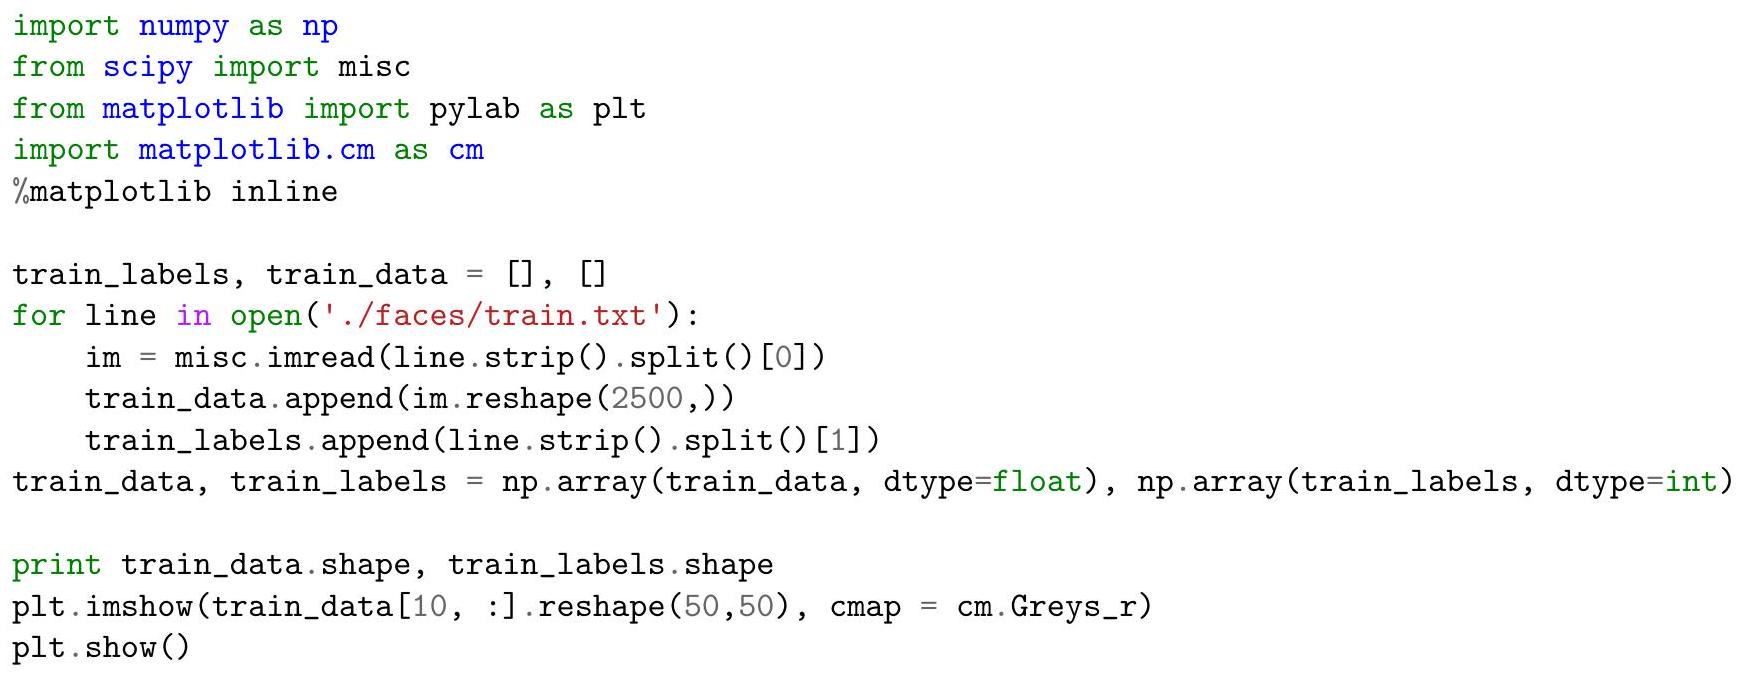
\includegraphics[max width=\textwidth]{2023_10_15_797733af37a95ba2c0b6g-2}
\end{center}

(c) (3 pts) Average Face. Compute the average face $\mu$ from the whole training set by summing up every row in $\mathbf{X}$ then dividing by the number of faces. Display the average face as a grayscale image.

(d) (3 pts) Mean Subtraction. Subtract average face $\mu$ from every row in $\mathbf{X}$. That is, $\mathbf{x}_{\mathbf{i}}:=\mathbf{x}_{\mathbf{i}}-$ $\mu$, where $\mathbf{x}_{\mathbf{i}}$ is the $i$-th row of $\mathbf{X}$. Pick a face image after mean subtraction from the new $\mathbf{X}$ and display that image in grayscale. Do the same thing for the test set $\mathbf{X}_{\text {test }}$ using the precomputed average face $\mu$ in (c).

(e) (10 pts) Eigenface. Perform eigendecomposition on $\mathbf{X}^{T} \mathbf{X}=\mathbf{V} \Lambda \mathbf{V}^{T}$ to get eigenvectors $\mathbf{V}^{T}$, where each row of $\mathbf{V}^{T}$ has the same dimension as the face image. We refer to $\mathbf{v}_{\mathbf{i}}$, the $i$-th row of $\mathbf{V}^{T}$, as $i$-th eigenface. Display the first 10 eigenfaces as 10 images in grayscale.

(f) (10 pts) Eigenface Feature. The top $r$ eigenfaces $\mathbf{V}^{T}[: r:$ : $]=\left\{v_{1}, v_{2}, \ldots, v_{r}\right\}^{T}$ span an $r$-dimensional linear subspace of the original image space called face space, whose origin is the average face $\mu$, and whose axes are the eigenfaces $\left\{\nu_{1}, \nu_{2}, \ldots, \nu_{r}\right\}$. Therefore, using the top $r$ eigenfaces $\left\{v_{1}, \nu_{2}, \ldots, v_{r}\right\}$, we can represent a 2500 -dimensional face image $\mathbf{z}$ as an $r$-dimensional feature vector $\mathbf{f}: \mathbf{f}=\mathbf{V}^{T}[: r::] \mathbf{z}=\left[\nu_{1}, \nu_{2}, \ldots, v_{r}\right]^{T} \mathbf{z}$. Write a function to generate $r$-dimensional feature matrix $\mathbf{F}$ and $\mathbf{F}_{\text {test }}$ for training images $\mathbf{X}$ and test images $\mathbf{X}_{\text {test }}$, respectively (to get $\mathbf{F}$, multiply $\mathbf{X}$ to the transpose of first $r$ rows of $\mathbf{V}^{T}, \mathbf{F}$ should have same number of rows as $\mathbf{X}$ and $r$ columns; similarly for $\mathbf{X}_{\text {test }}$ ).

(g) (10 pts) Face Recognition. For this problem, you are welcome to use libraries such as scikit learn to perform logistic regression. Extract training and test features for $r=10$. Train a Logistic Regression model using $\mathbf{F}$ and test on $\mathbf{F}_{\text {test }}$. Report the classification accuracy on the test set. Plot the classification accuracy on the test set as a function of $r$ when $r=1,2, \ldots, 200$. Use "one-vs-rest" logistic regression, where a classifier is trained for each possible output label. Each classifier is trained on faces with that label as positive data and all faces with other labels as negative data. sklearn calls this the "ovr" mode.

(h) (5 pts) Low-Rank Data Loss. These feature matrices $\mathbf{F}$ can be mapped back to their original dimensions; however, information is lost in the process and only approximations $\mathbf{X}^{\prime}$ will be recovered. This is done by multiplying the feature matrices $\mathbf{F}$ once again by the first $r$ rows of $\mathbf{V}^{T}$. Plot the average Frobenius distance $d\left(\mathbf{X}, \mathbf{X}^{\prime}\right)=\sqrt{\operatorname{tr}\left(\left(\mathbf{X}-\mathbf{X}^{\prime}\right)^{T}\left(\mathbf{X}-\mathbf{X}^{\prime}\right)\right)}$ between the original data $\mathbf{X}$ and their approximations $\mathbf{X}^{\prime}$, over $r=1,2, \ldots, 200$.

\begin{enumerate}
  \setcounter{enumi}{1}
  \item Implement EM algorithm. (40 pts) In this problem, you will implement a bimodal GMM model fit using the EM algorithm. Bimodal means that the distribution has two peaks, or that the data is a mixture of two groups. If you want, you can assume the covariance matrix is diagonal (i.e. it has the form $\operatorname{diag}\left(\sigma_{1}^{2}, \sigma_{2}^{2}, \ldots, \sigma_{d}^{2}\right)$ for scalars $\left.\sigma_{i}\right)$ and you can randomly initialize the parameters of the model.
\end{enumerate}

You will need to use the Old Faithful Geyser Dataset. The data file contains 272 observations of the waiting time between eruptions and the duration of each eruption for the Old Faithful geyser in Yellowstone National Park.

You should do this without calling the Gaussian Mixture library in scikit learn. You can use numpy or scipy for matrix calculation or generating Gaussian distributions.

(a) (2 pts) Treat each data entry as a 2 dimensional feature vector. Parse and plot all data points on 2-D plane.

(b) (3 pts) Recall that EM learns the parameter $\theta$ of a Gaussian mixture model $P_{\theta}(x, z)$ over a dataset $D=\left\{x^{(i)} \mid i=1,2, \ldots n\right\}$ by performing the E-step and the M-step for $t=0,1,2, \ldots$. We repeat the E-step and and $\mathrm{M}$-step until convergence.

In the E-step, for each $x^{(i)} \in D$, we compute a vector of probabilities $P_{\theta_{t}}(z=k \mid x)$ for the event that each $x^{(i)}$ originates from a cluster $k$ given the current set of parameters $\theta_{t}$.

Write the expression for $P_{\theta_{t}}(z=k \mid x)$, which is the posterior of each data point $x^{(i)}$. Recall that by Bayes' rule,

$$
P_{\theta_{t}}(z=k \mid x)=\frac{P_{\theta_{t}}(z=k, x)}{P_{\theta_{t}}(x)}=\frac{P_{\theta_{t}}(z=k, x)}{\sum_{l=1}^{K} P_{\theta_{t}}(x \mid z=l) P_{\theta_{t}}(z=l)} .
$$

Note that we have seen this formula in class. We are asking you to write it down and try to understand and it before implementing it in part (e).

(c) (5 pts) In the M-step, we compute new parameters $\theta_{t+1}$. Our goal is to find $\mu_{k}, \Sigma_{k}$ and $\phi_{k}$ that optimize

$$
\max _{\theta}\left(\sum_{k=1}^{K} \sum_{x \in D} P_{\theta_{t}}\left(z_{k} \mid x\right) \log P_{\theta}\left(x \mid z_{k}\right)+\sum_{k=1}^{K} \sum_{x \in D} P_{\theta_{t}}\left(z_{k} \mid x\right) \log P_{\theta}\left(z_{k}\right)\right)
$$

Write down the formula for $\mu_{k}, \Sigma_{k}$, and for the parameters $\phi$ at the M-step (we have also seen these formulas in class).

(d) (25 pts) Implement and run the EM algorithm. Specifically:

i. (10 pts) Implement the EM algorithm from scratch (e.g., in Python and numpy).

ii. (5 pts) Choose a termination criterion for when the algorithm stops repeating the E-step and the M-step. State your termination criterion and explain the reasoning behind it.

iii. (10 pts) Plot the trajectories of the two mean vectors $\left(\mu_{1}\right.$ and $\left.\mu_{2}\right)$ in two dimensions as they change over the course of running EM. You might want to use a scatter plot for this.

(e) (5 pts) If you were to run $K$-means clustering instead of the EM algorithm you just implemented, do you think you will get different clusters? You are welcome to experiment with $K$-means clustering on the same dataset with $K=2$. (The KNN library from scikit learn is a good way to try). Comment on why do you think the results will or will not change. .

\begin{enumerate}
  \setcounter{enumi}{2}
  \item Kernel Density Estimation. (12pts) For this question, you may use existing libraries, or you may implement the method yourself in numpy. Consider the following set of $n=10$ samples drawn from a distribution.
\end{enumerate}

$$
\begin{array}{llllllllll}
26 & 30 & 27 & 18 & 75 & 66 & 73 & 63 & 56 & 83
\end{array}
$$

(a) (4 pts) Let $\tilde{p}(x)=\sum_{i=1}^{n} K\left(x^{(i)}, x ; \delta\right)$ be a kernel density estimate of the data distribution with a Gaussian kernel $K(x, z ; \delta) \propto \exp \left(\frac{-\|x-z\|^{2}}{2 \delta}\right)$ and a bandwidth parameter $\delta>0$. Plot the density estimate $\tilde{p}(x)$ of the above dataset as a function of $x$ on an interval containing the data using two choices of bandwidth $\delta=100$ and $\delta=10$. For this and the rest of the problem, $\tilde{p}$ can be either a normalized or an unnormalized probability. (b) (2 pts) Explain which of the above two choices of $\delta$ you think is better. Name at least one method for choosing the better $\delta$ out of the two options.

(c) (2 pts) Suppose you observe two new samples: 30 and 95. Compute and report their (possibly unnormalized) probability $\tilde{p}(x)$ for both $\delta=100$ and $\delta=10$.

(d) (2 pts) Provide one possible rule by which a kernel density estimate can be used to either accept a point as being part of the data distribution or reject it for being an outlier. Provide one scenario in which this strategy might not work.

(e) (2 pts) Let's say that instead of a Gaussian kernel, a Tophat kernel $(K(x, z ; \delta)=1$ if $\|x-z\| \leq \delta / 2$ else 0 ) is chosen for modeling. Plot the Tophat density estimate $\tilde{p}(x)$ of the dataset as a function of $x$ on an interval containing the data using $\delta=10$. Give one example of a shortcoming of the Tophat kernel density estimate for outlier detection relative to the Gaussian kernel.

\section{WRITTEN EXERCISES}
\begin{enumerate}
  \item K-means clustering. (10 pts) For a dataset consisting of $n$ points, $x^{(i)} \in \mathbb{R}^{d}$ for $i=1,2, \ldots n$, the goal of K-means clustering is to find a function $f: \mathbb{R}^{d} \rightarrow\{1,2, \ldots, K\}$ that assigns each point to one of $K$ clusters. Each cluster is represented by a centroid, $c^{(k)} \in \mathbb{R}^{d}$ for $k=1,2, \ldots, K$. Recall from the lecture on unsupervised learning that the K-means objective is optimized by an iterative process. For each iteration $t$, let $f_{t}$ denote the cluster assignment function and $c_{t}^{(k)}$ denote the $k^{\text {th }}$ centroid. Then, at each iteration $t$, we perform two steps: (1) update cluster assignments $f_{t}\left(x^{(i)}\right)$ for each point $x^{(i)}$ and (2) update centroids $c_{t}^{(k)}$ for each cluster $k=1,2, \ldots, K$ :
\end{enumerate}

Initialization: set centroids $c_{0}^{(k)}$ randomly or using an initialization heuristic. For $t=1,2, \ldots$ until K-Means converges, do:

Step 1. Update cluster assignments such that $f_{t}\left(x^{(i)}\right)=\operatorname{argmin}_{k}\left\|x^{(i)}-c_{t-1}^{(k)}\right\|_{2}$ is the cluster of the closest centroid to $x^{(i)}$, where $\|\cdot\|_{2}$ denotes Euclidean norm.

Step 2. Set each centroid $c_{t}^{(k)}$ to be the average of its cluster. Letting $S^{(k)}=\left|\left\{x^{(i)} \mid f_{t}\left(x^{(i)}\right)=k\right\}\right|$ be the number of points assigned to cluster $k$, we refit centroids as follows:

$$
c_{t}^{(k)}=\frac{1}{S^{(k)}} \sum_{i: f_{t}\left(x^{(i)}\right)=k} x^{(i)}
$$

Letting $c_{t}$ (i.e., without any superscript) be a shorthand representation for all $K$ centroids $\left\{c_{t}^{(1)}, c_{t}^{(2)}, \ldots, c_{t}^{(K)}\right\}$, we can express the K-means optimization objective at each time $t$ as follows:

$$
J\left(c_{t}, f_{t}\right)=\sum_{i=1}^{n}\left\|x^{(i)}-c_{t}^{\left(f_{t}\left(x^{(i)}\right)\right)}\right\|_{2}
$$

where $c_{t}^{\left(f_{t}\left(x^{(i)}\right)\right)}$ denotes "the centroid for the cluster assignment of $x^{(i)}$ at time $t$ ". In this question, we want to prove that K-means optimization is guaranteed to converge. In other words, we want to prove that the K-means objective $J\left(c_{t}, f_{t}\right)$ is monotonically decreasing after each step of K-means optimization procedure:

$$
J\left(c_{t}, f_{t}\right) \leq J\left(c_{t-1}, f_{t-1}\right)
$$

If we prove this, then convergence follows from the monotone convergence theorem, which states that a monotonically decreasing sequence with a lower bound (the bound is $J\left(c_{t}, f_{t}\right) \geq 0, \forall t$, in our case) is guaranteed to converge.

(a) (5 pts) Show that $J\left(c_{t-1}, f_{t}\right) \leq J\left(c_{t-1}, f_{t-1}\right)$. This is equivalent to proving that the K-means objective is decreasing after updating cluster assignments (but before updating the centroids).

(b) (5 pts) Show that $J\left(c_{t}, f_{t}\right) \leq J\left(c_{t-1}, f_{t}\right)$. This is equivalent to proving that the K-means objective is decreasing after refitting centroids.

\begin{enumerate}
  \setcounter{enumi}{1}
  \item Local Optima in K-means. (5pts) Depending on initialization, K-means can get stuck on local optima. Construct an example dataset ( $>3$ points), and provide two different initializations for it such that K-means would return different final clusterings on it.
\end{enumerate}

\end{document}